% Sturm.tex
% Copyright (c) Sergey Strukov. All rights reserved. This is a public document. You can freely distribute and use it, providing the authorship and the copyright note is unchanged.

\input ../SSCommon.tex

\begin{document}
\selectlanguage{russian}
    
\SScover
    
\SStitle{Теорема Штурма}

Теорема Штурма --- красивая элементарная теорема школьного уровня. Она позволяет найти число корней данного полинома с вещественными коэффициентами на заданном интервале.
С её помощью можно локализовать корни вещественных полиномов и находить хорошие приближения к ним.

\vspace

\SSbullet 

\begin{tikzpicture}
    \draw[thick,->] (0,-2) -- (0,2) node[anchor=north west] {\(y\)};
    \draw[thick,->] (-2,0) -- (2,0) node[anchor=north west] {\(x\)};
    \draw (1,1) node[anchor=south west] {\(0\)};
    \draw (1,-1) node[anchor=north west] {\(1\)};
    \draw (-1,1) node[anchor=south east] {\(1\)};
    \draw (-1,-1) node[anchor=north east] {\(0\)};
\end{tikzpicture}

\SSsect[def] Функция \( \sigma: \xR^* \times \xR^* \rightarrow \{0,1\} \) определена как
\[ \sigma(x,y) := 
   \begin{cases} 
       1, & sign(x) = sign(y) \\ 
       0, & sign(x) \neq sign(y)
   \end{cases} 
\]

\SSsect \( \sigma(x,y) = \sigma(y,x) \)

\SSsect \( \sigma(x,y) = \sigma(sign(x),y) = \sigma(sign(x),sign(y)) \)

\SSsect \( \sigma(-x,y) = 1 - \sigma(x,y) \)

\SSsect[def] \( \sigma(x_1,\dots,x_n) \) , \( x_1,\dots,x_n \in \xR^* \) , \( n \geqslant 1 \)
\[ \sigma(x_1,\dots,x_n) := \sum_{k=1}^{n-1} \sigma(x_k,x_{k+1})
\]
--- число перемен знака (Ч.П.З.)

\SSsect Индуктивно,
\begin{itemize}[label=]
\item \( \sigma(x_1) = 0 \) ,
\item \( \sigma(x_1,\dots,x_n) = \sigma(x_1,x_2) + \sigma(x_2,\dots,x_n) \) , \( n \geqslant 2 \) .
\end{itemize}

\vspace

\SSbullet

В этом пункте \( f,g \in \xR[T] \) .

\SSsect Пусть \( f \) и \( g \) не имеют общих вещественных корней. 
Пусть \( a,b \in \xR \) , \( a < b \) .

\SSsect Пусть \( a,b \) --- не корни \( f \) или \( g \) .
Т.е. \( f(a),g(a),f(b),g(b) \in \xR^* \) .

\SSsect[def] Определим \( \varphi(t) := \sigma(f(t),g(t)) \) , \( t \in \xR \) .
Тогда \( \varphi \) определена вне (конечного) множества корней \( f \) или \( g \) ,
например, в \( a \) и \( b \) .

\SSsect Функция \( \varphi(t) \) локально постоянна. Это вытекает из непрерывности \( f(t) \) ,
\( g(t) \) и локального постоянcтва \( \sigma(x,y) \) .

\vspace
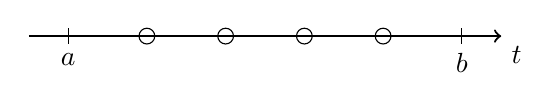
\begin{tikzpicture}
\draw[thick,->] (0,0) -- (6,0) node[anchor=north west] {\(t\)};    
\draw (0.5,0.1) -- (0.5,-0.1) node[anchor=north] {\(a\)};
\draw (5.5,0.1) -- (5.5,-0.1) node[anchor=north] {\(b\)};
\draw[] (1.5,0) circle [radius=0.1];
\draw[] (2.5,0) circle [radius=0.1];
\draw[] (3.5,0) circle [radius=0.1];
\draw[] (4.5,0) circle [radius=0.1];
\end{tikzpicture}


\SSsect[def] Определим \( \delta(t) := \varphi(t+0) - \varphi(t-0) \in \{-1,0,1\} \) --- 
функция скачков \( \varphi \) .

\SSsect \( \delta(t) = 0 \) вне корней \( f \) или \( g \) .

\SSsect[!!] Главная теорема:
\[ \varphi(b) - \varphi(a) = \sum_{ a<t<b \enspace \delta(t) \neq 0 } \delta(t) \]

\def\Symbol#1#2{ \left( \frac{#1}{#2} \right)^b_a }

\SSsect[def] Определим символ
\[ \Symbol{f}{g} := \sum_{ a<t<b \enspace g(t)=0 } \delta(t) \]

\SSsect \( \varphi \) и \( \delta \) для пар \( (f,g) \) и \( (g,f) \) одинаковы.

\SSsect[!!] Закон взаимности:
\[ \Symbol{f}{g} + \Symbol{g}{f} = \varphi(b)-\varphi(a) \]

\SSsect Если заменить \( f \) на \( -f \) , то \( \varphi \) превратиться в \( 1-\varphi \) , а \( \delta \) в \( -\delta \) .

\SSsect[!] Нечётность:
\[ \Symbol{-f}{g} = - \Symbol{f}{g} \]

\SSsect[!] Модулярность. Если заменить \( f \) на полином \( h \in \xR[T] \) , такой, что
\( g(t) = 0 \Rightarrow h(t) = f(t) \) , то значения \( \delta(t) \) не изменяться в точках
\( \SSet{ t\in \xR }{ g(t) = 0 } \) . Поэтому
\[ \Symbol{h}{g} = \Symbol{f}{g} \]
В частности, это верно, если \( h=f-qg \) . Для доказательства см. картинку:

\vspace

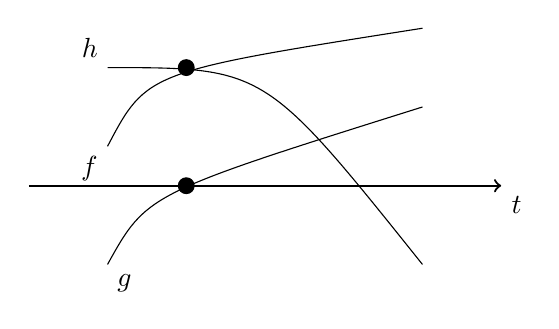
\begin{tikzpicture}
\draw[thick,->] (0,0) -- (6,0) node[anchor=north west] {\(t\)};    
\draw[fill,black] (2,0) circle [radius=0.1];
\draw[fill,black] (2,1.5) circle [radius=0.1];
\draw (1,-1) node[anchor=north west] {\(g\)} .. controls (1.5,-0.1) .. (5,1) ;
\draw (1,0.5) node[anchor=north east] {\(f\)} .. controls (1.5,1.45) .. (5,2) ;
\draw (1,1.5) node[anchor=south east] {\(h\)} .. controls (3,1.5) .. (5,-1) ;
\end{tikzpicture}

Пояснение, вблизи точки \( t \) значения \( f\) и \( h \) имеют одинаковый знак, \( sign(f) = sign(h) \) , поэтому две версии \( \varphi \) совпадают, а, значит, совпадают и две версии \( \delta \).

\vspace

\SSresume

\SSsect 
\[ \Symbol{f}{g} \in \xZ \]

\SSsect
\[ \Symbol{-f}{g} = - \Symbol{f}{g} \]

\SSsect
\[ g(t) = 0 \Rightarrow h(t) = f(t) \]
\[ \Downarrow \]
\[ \Symbol{h}{g} = \Symbol{f}{g} \]

\SSsect
\[ \Symbol{f}{g} + \Symbol{g}{f} = \varphi(b)-\varphi(a) = \sigma(f(b),g(b)) - \sigma(f(a),g(a)) \]

\SSsect Если \( g \) не имеет вещественных корней, то
\[ \Symbol{f}{g} = 0 \]

\SSbullet

\begin{center}
    \( f \) , \( g \) , \( a \) , \( b \) --- такие же, как и выше
\end{center}

\SSsect Определим последовательность
\begin{itemize}[label=]
\item \( f_0 := f \)
\item \( f_1 := g \)
\item \( \dots \)
\item \( f_k = f_{k+1} q_k - f_{k+2} \) , \( k \geqslant 0 \) --- деление с остатком
\item \( \dots \)
\item \( f_{n-1} = f_n q_{n-1}\)
\end{itemize}

\SSsect 
\begin{itemize}[label=]
\item \( f_0,f_1,\dots,f_n \) --- \underline{ряд Штурма}, \( n \geqslant 1 \)   
\item \( deg(f_{k+1}) < deg(f_k) \) , \( 1 \leqslant k < n \)  
\item \( f_0,\dots,f_n \in (f_n) \) , \( f_n=(f,g) \)  
\item \( f_n \) не имеет вещественных корней  
\end{itemize}

\SSsect[!] Допустим, что члены ряда Штурма не обращаются в нуль в точках \( a \) и \( b \) .
Тогда
\[ \Symbol{f}{g} = \sigma(f_1(a),\dots,f_n(a)) - \sigma(f_1(b),\dots,f_n(b)) \]

\SSproof

\[ \Symbol{f}{g} = \Symbol{f_0}{f_1} \]

\[ \Symbol{f_k}{f_{k+1}} = \Symbol{-f_{k+2}}{f_{k+1}} = - \Symbol{f_{k+2}}{f_{k+1}} = \]

\[ + \Symbol{f_{k+1}}{f_{k+2}} + \sigma(f_{k+1}(a),f_{k+2}(a))-\sigma(f_{k+1}(b),f_{k+2}(b)) \]

\[ \Symbol{f}{g} = \Symbol{f_{n-1}}{f_{n}} + \sigma(f_1(a),f_2(a))-\sigma(f_1(b),f_2(b)) + \dots + \sigma(f_{n-1}(a),f_{n}(a))-\sigma(f_{n-1}(b),f_{n}(b)) = \]

\[ 0 + \sigma(f_1(a),\dots,f_n(a)) - \sigma(f_1(b),\dots,f_n(b)) \]

\SSendp

\vspace

\SSbullet

\begin{center}
Пусть \( f \in \xR[T] \) --- полином без кратных корней

\( a,b \in \xR \) , \( a<b \) ,

\( a \) и \( b \) --- не корни \( f \) или \( f' \)
\end{center}

\SSsect \( (f,f')=1 \) , \( f \) и \( f' \) не имеют общих корней

\SSsect[!]
\[ \Symbol{f'}{f} = - \text{ число корней } f \text{ на } (a,b) \] 

\SSproof

\vspace
Достаточно доказать, что \( f(t) = 0  \Rightarrow \delta(t) = -1 \) .

Для доказательства см. следующие картинки:

\vspace

\begin{tikzpicture}
    \draw[thick,->] (0,0) -- (6,0) node[anchor=north west] {\(t\)};    
    \draw[fill,black] (2,0) circle [radius=0.1];
    \draw[fill,black] (2,1.5) circle [radius=0.1];
    \draw (1,-1) node[anchor=north west] {\(f\)} .. controls (1.5,-0.1) .. (5,1) ;
    \draw (1,0.5) node[anchor=north east] {\(f'\)} .. controls (1.5,1.45) .. (5,2) ;
\end{tikzpicture}

\vspace

\( \varphi(t+0) = 0 \) , \( \varphi(t-0) = 1 \) , \( \delta(t) = -1 \)

\vspace

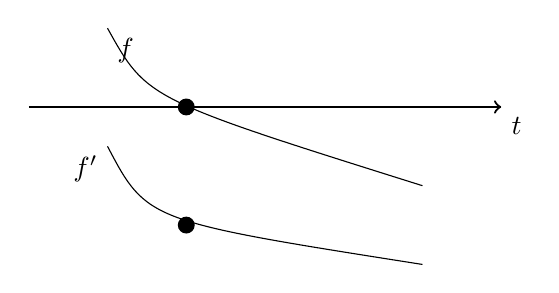
\begin{tikzpicture}
    \draw[thick,->] (0,0) -- (6,0) node[anchor=north west] {\(t\)};    
    \draw[fill,black] (2,0) circle [radius=0.1];
    \draw[fill,black] (2,-1.5) circle [radius=0.1];
    \draw (1,1) node[anchor=north west] {\(f\)} .. controls (1.5,0.1) .. (5,-1) ;
    \draw (1,-0.5) node[anchor=north east] {\(f'\)} .. controls (1.5,-1.45) .. (5,-2) ;
\end{tikzpicture}

\vspace

\( \varphi(t+0) = 0 \) , \( \varphi(t-0) = 1 \) , \( \delta(t) = -1 \)

\vspace

Пояснение, \( sign(f(t+0)) = sign(f'(t)) \) , \( sign(f(t-0)) = - sign(f'(t)) \) .

\SSendp

\SSsect[!!] \underline{Теорема Штурма}

\vspace

Пусть \( f_0 = f \) , \( f_1=f' \) , \( \dots \) , \( f_n \) , \( n \geqslant 1 \) --- ряд Штурма.
Пусть члены ряда не обращаются в нуль в точках \( a \) и \( b \) .
Тогда 
\[ \text{ число корней } f \text{ на } (a,b) = \sigma(f_0(a),\dots,f_n(a)) - \sigma(f_0(b),\dots,f_n(b)) \]

\SSproof

\[ - \Symbol{f'}{f} = \Symbol{f}{f'} + \sigma(f(a),f'(a)) - \sigma(f(b),f'(b)) = \]

\[ \sigma(f(a),f'(a)) + \sigma(f_1(a),\dots,f_n(a)) - \sigma(f(b),f'(b)) - \sigma(f_1(b),\dots,f_n(b)) \]

\SSendp

\SSsect Пусть \( g(t) = Gt^n+\dots \) --- полином, \( Gt^n \) --- его старший член.
Тогда \( sign(g(a)) = sign(G)(-1)^n \) для \( a \rightarrow -\infty \) ,
\( sign(g(b)) = sign(G) \) для \( b \rightarrow +\infty \) . 
Будем писать \( sign(g(-\infty)) := sign(G)(-1)^n \) и \( sign(g(+\infty)) := sign(G) \) .

\SSsect \underline{Следствие}

\vspace

Пусть \( f_0 = f \) , \( f_1=f' \) , \( \dots \) , \( f_n \) , \( n \geqslant 1 \) --- ряд Штурма.

Тогда 
\[ \text{ число корней } f = \sigma(sign(f_0(-\infty)),\dots,sign(f_n(-\infty))) - \sigma(sign(f_0(+\infty)),\dots,sign(f_n(+\infty))) \]

\SSsect \underline{Теорема Штурма\(+\)}

\vspace

Пусть \( f_0 = f \) , \( f_1=f' \) , \( \dots \) , \( f_n \) , \( n \geqslant 1 \) --- ряд Штурма. Пусть \( f \) не обращается в нуль в точках \( a \) и \( b \) .
Тогда 
\[ \text{ число корней } f \text{ на } (a,b) = \sigma(f_0(a),\dots,f_n(a)) - \sigma(f_0(b),\dots,f_n(b)) \]
При этом если один из аргументов \( \sigma \) равен нулю, его надо просто вычеркнуть.

\end{document}

